%%%%%%%%%%%%%%%%%%%%%%%%%%%%%%%%%%%%%%%%%%%%%%%%%%%%%%%%%%%%%%%%%
% MUW Presentation
% LaTeX Template
% Version 1.0 (27/12/2016)
%
% License:
% CC BY-NC-SA 4.0 (http://creativecommons.org/licenses/by-nc-sa/3.0/)
%
% Created by:
% Nicolas Ballarini, CeMSIIS, Medical University of Vienna
% nicoballarini@gmail.com
% http://statistics.msi.meduniwien.ac.at/
%
% Customized for UAH by:
% David F. Barrero, Departamento de Automática, UAH
%%%%%%%%%%%%%%%%%%%%%%%%%%%%%%%%%%%%%%%%%%%%%%%%%%%%%%%%%%%%%%%%%

\documentclass[10pt,compress]{beamer} % Change 10pt to make fonts of a different size
\mode<presentation>

\usepackage[spanish]{babel}
\usepackage{fontspec}
\usepackage{tikz}
\usepackage{etoolbox}
\usepackage{xcolor}
\usepackage{xstring}
\usepackage{listings}

\usetheme{UAH}
\usecolortheme{UAH}
\setbeamertemplate{navigation symbols}{} 
\setbeamertemplate{caption}[numbered]

%%%%%%%%%%%%%%%%%%%%%%%%%%%%%%%%%%%%%%%%%%%%%%%%%%%%%%%%%%%%%%%%%
%% Presentation Info
\title[Getting started]{Getting started}
\author{}
\institute{\asignatura}
\date{}
%%%%%%%%%%%%%%%%%%%%%%%%%%%%%%%%%%%%%%%%%%%%%%%%%%%%%%%%%%%%%%%%%


%%%%%%%%%%%%%%%%%%%%%%%%%%%%%%%%%%%%%%%%%%%%%%%%%%%%%%%%%%%%%%%%%
%% Descomentar para habilitar barra de navegación superior
\ponerNavegacion
%%%%%%%%%%%%%%%%%%%%%%%%%%%%%%%%%%%%%%%%%%%%%%%%%%%%%%%%%%%%%%%%%

%%%%%%%%%%%%%%%%%%%%%%%%%%%%%%%%%%%%%%%%%%%%%%%%%%%%%%%%%%%%%%%%%
%% Configuración de logotipos en portada
%% Opacidad de los logotipos
\newcommand{\opacidad}{1}
%% Descomentar para habilitar logotipo en pié de página de portada
\renewcommand{\logoUno}{Images/isg.png}
%% Descomentar para habilitar logotipo en pié de página de portada
%\renewcommand{\logoDos}{Images/CCLogo.png}
%% Descomentar para habilitar logotipo en pié de página de portada
%\renewcommand{\logoTres}{Images/ALogo.png}
%% Descomentar para habilitar logotipo en pié de página de portada
%\renewcommand{\logoCuatro}{Images/ELogo.png}
%%%%%%%%%%%%%%%%%%%%%%%%%%%%%%%%%%%%%%%%%%%%%%%%%%%%%%%%%%%%%%%%%

%%%%%%%%%%%%%%%%%%%%%%%%%%%%%%%%%%%%%%%%%%%%%%%%%%%%%%%%%%%%%%%%%
%% FOOTLINE
%% Comment/Uncomment the following blocks to modify the footline
%% content in the body slides. 


%% Option A: Title and institute
\footlineA
%% Option B: Author and institute
%\footlineB
%% Option C: Title, Author and institute
%\footlineC
%%%%%%%%%%%%%%%%%%%%%%%%%%%%%%%%%%%%%%%%%%%%%%%%%%%%%%%%%%%%%%%%%

\begin{document}

%%%%%%%%%%%%%%%%%%%%%%%%%%%%%%%%%%%%%%%%%%%%%%%%%%%%%%%%%%%%%%%%%
% Use this block for a blue title slide with modified footline
{\titlepageBlue
    \setbeamertemplate{headline}{}
	\setbeamercolor{frametitle}{bg=black}
	\setbeamercolor{normal text}{bg=black}
    \begin{frame}
        \titlepage
    \end{frame}
}

\begin{frame}[plain]{}
   \begin{block}{Objectives}
      \begin{enumerate}
         \item Understand the concept of programming language
         \item Introduce interpreted and compiled languages
         \item Describe the Java Virtual Machine
         \item First contact with Java code
      \end{enumerate} 
   \end{block}

   \begin{block}{Bibliography}
      \begin{enumerate}
          \item The Java\textsuperscript{TM} Tutorials. Oracle. \href{https://docs.oracle.com/javase/tutorial/}{(Link)}
      \end{enumerate} 
   \end{block}


\end{frame}

{
\eliminarNavegacion
\begin{frame}[shrink]{Table of Contents}
 \frametitle{Table of Contents}
 \tableofcontents
  % You might wish to add the option [pausesections]
\end{frame}
}

\section{Programming languages}

\begin{frame}[plain]{Programming languages (I)}
	\textbf{Programming language}: A formal language designed to communicate instructions to a machine

	\vspace{-0.2cm}
   	 	\begin{figure}[t]
		\begin{center}
		    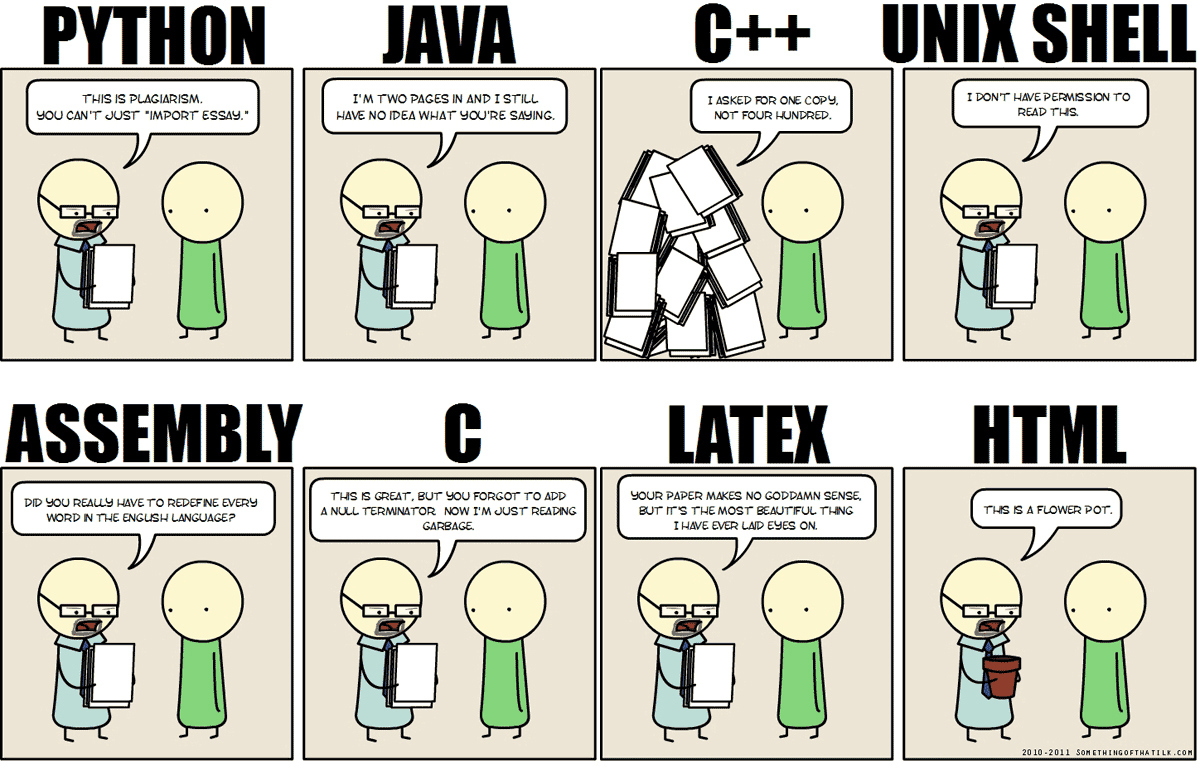
\includegraphics[width=\linewidth]{figs/lenguajes.jpg}
		\end{center}
   	 	\end{figure}

\end{frame}

\begin{frame}{Programming languages (II)}
	Languages types
	\begin{itemize}
		\item \textit{Compiled}: C, C++, Pascal, ...
		\item \textit{Interpreted} (\alert{scripts}): Python, Perl, PHP, ...
 	\end{itemize}

	\begin{columns}
 	   \column{.50\textwidth}
		\begin{tabular}{|l|l|l|}
		\hline
		      		& Compiled 	& Interpreted  \\\hline
		Speed 		& Fast 	 	& Slow 		\\
		Development	& Slow 	 	& Fast 		\\
		Abstraction & Low/High	& High 		\\
		Flexibility & Low		& High 		\\
		Project size& Large		& Small 	\\\hline
		\end{tabular}
 	   \column{.50\textwidth}
		\begin{figure}[t]
		\begin{center}
		    
\includegraphics[width=0.7\linewidth]{figs/wordmap.png}
		\end{center}
   	 	\end{figure}
\end{columns}
\end{frame}

\section{Overview of Java}

\subsection[Why Java?]{Why Java?}
\begin{frame}{Overview of Java}{Why Java? (I)}
	\begin{itemize}
	\item Widely used in the industry
		\begin{itemize}
		\item Good point in your CV!
		\end{itemize}
	\item Large number of domains
		\begin{itemize}
		\item Desktop applications, servers, embedded systems, tablets, mobiles, ...
		\item Videogames industry shifts to wider range of platforms
		\item Java videogames for mobile platforms
		\end{itemize}
	\item Clean and elegant object-oriented language
	\item High level (do more with less code)
	\item Syntax similar to other languages
	\item Availability of videogames source code
  	\end{itemize}
\end{frame}

\begin{frame}{Overview of Java}{Why Java? (II)}
    \begin{columns}
 	   \column{.50\textwidth}
	   \begin{block}{Advantages}
  		\begin{itemize}
		\item Device independent
		\item Safety
		\item Java standards
		\item Object-oriented
		\item Many applications
  		\end{itemize}
		\end{block}
 	   \column{.50\textwidth}
		\begin{block}{Disadvantages}
		\begin{itemize}
		\item Slower execution
		\item Difficult device specific features
		\item JVM availability
		\item Huge ecosystem
  		\end{itemize}
		\end{block}
	\end{columns}
\end{frame}


\subsection[About the Java technology]{About the Java technology}
\begin{frame}{Overview of Java}{About the Java technology}
    \begin{columns}
 	   \column{.70\textwidth}
  		  \begin{itemize}
			\item Java was created by Sun Microsystems
		   	\begin{itemize}
				\item Now Java belongs to Oracle
		  	\end{itemize}

			\item History
		   	\begin{itemize}
				\item 1.0 (1996), 1.1 (1997), 1.2 (1998), 1.3 (2000), 1.4 (2002)
				\item 5 (2004), 6 (2006), 7 (2011), 8 (2014)
		  	\end{itemize}
		\item Java is a programming language and a platform
	    	\begin{itemize}
			\item Programming language: Like C or C++
			\item Platform: Where programs run, including hardware and operating system
	    	\end{itemize}
		  	\end{itemize}
   	 \column{.30\textwidth}
   	 	\begin{figure}[t]
		\begin{center}
		    
\includegraphics[width=0.6\linewidth]{figs/java}\\
			\bigskip
		    
\includegraphics[width=0.6\linewidth]{figs/Sun}\\
			\bigskip
		    
\includegraphics[width=0.6\linewidth]{figs/oracle}
		\end{center}
   	 	\end{figure}
    \end{columns}

\end{frame}

\subsection[Java as programming language]{Java as programming language}
\begin{frame}{Overview of Java}{Java as programming language (I)}
	\begin{center}
	The standard way\\
	\bigskip
	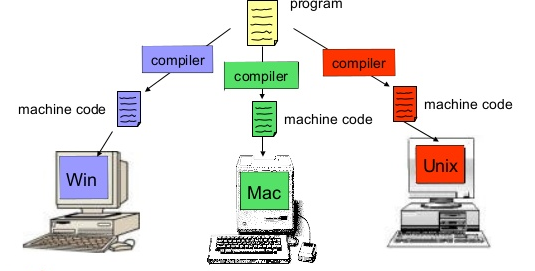
\includegraphics[width=0.8\linewidth]{figs/compilacion}\\
	\scriptsize{\href{http://es.slideshare.net/darokoblog/an-introduction-to-java-programming-language-forbeginnersjava-programming-tutorials}{(Source)}}
	\end{center}
\end{frame}

\begin{frame}{Overview of Java}{Java as programming language (II)}
	\begin{center}
	The Java way: \textit{Write once, run anywhere}\\
	\smallskip
	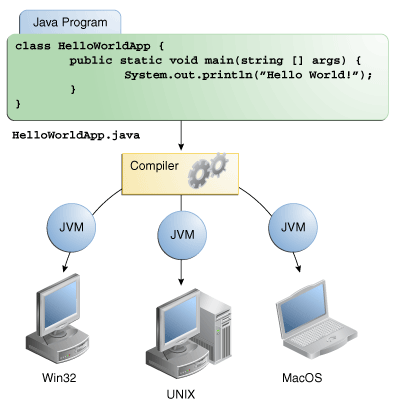
\includegraphics[width=0.5\linewidth]{figs/helloWorld}\\
	\scriptsize{\href{http://docs.oracle.com/javase/tutorial/getStarted/intro/definition.html}{(Source)}}
	\end{center}
\end{frame}

\begin{frame}{Overview of Java}{Java as programming language (III)}
	\begin{center}
	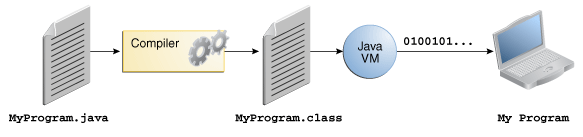
\includegraphics[width=\linewidth]{figs/getStarted-compiler}\\
	\scriptsize{\href{http://docs.oracle.com/javase/tutorial/getStarted/intro/definition.html}{(Source)}}
	\end{center}
	\bigskip

	\normalsize{\textbf{*.java:} Source code file}\\
	\normalsize{\textbf{*.class:} Bytecode file}\\
	\normalsize{\textbf{Bytecode:} Machine language of the Java Virtual Machine (JVM)}
\end{frame}
\subsection[Java as platform]{Java as platform}
\begin{frame}{Overview of Java}{Java as platform}
	\begin{itemize}
	\item A platform is all the required infraestructure to run a program
	\item Usually, hardware (CPU) + software (OS)
		\begin{itemize}
		\item In Java all the platform uses to be software
		\end{itemize}
	\item Two components: JVM (\textit{Java Virtual Machine}) and API (\textit{Application Programming Interface})
	\end{itemize}
	\centering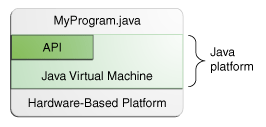
\includegraphics[width=0.5\linewidth]{figs/getStarted-jvm}\\
\end{frame}

\subsection[Acronyms]{Acronyms}
\begin{frame}{Overview of Java}{Acronyms}
	JSE: Java Standard Edition (Java Virtual Machine, JVM)\\
	JDK: Java Developer Kit (Compiler + JVM)\\
	J2EE: Java Enterprise Edition\\
	J2ME (now Java ME): Java Micro Edition\\
	Others: AWT, Swing, Ajax, EJB, HPJ, JAX, JDBC, JSP, Servlet, SAX, JDOM, ...
\end{frame}

\section[Hello world!]{Hello world!}
\begin{frame}{Hello World!}{Hello world! (I)}
	\vspace{-0.2cm}
	\begin{block}{HelloWorld.java}
		\lstinputlisting{code/HelloWorld.java}
	\end{block}

	Procedure:
	\begin{enumerate}
		\item Compile: \texttt{javac HelloWorld.java}
		\item Run: \texttt{java HelloWorld}
	\end{enumerate}
\end{frame}

\begin{frame}{Hello World!}{Hello world! (II)}
	\begin{itemize}
		\item Java is an evolution of C: Almost same syntaxis
     	\item Entry point in \texttt{main()}
		\item \texttt{System.out.println()} prints a string
		\item // and /* ... */ are comments
		\item /** ... */ is a \alert{javadoc} comment
		\item Java ignores the end of line
	    	\begin{itemize}
		 	\item `;' marks the end of instruction
 		 	\end{itemize}
		\item Keyword \texttt{class} begins the class definition
	    	\begin{itemize}
		 	\item Class name and file name \textit{must} be equal!
 		 	\end{itemize}
	\end{itemize}
\end{frame}

\section[Example]{Example}
\begin{frame}{Example}
	\vspace{-0.2cm}
	\begin{block}{Hello.java}
		\lstinputlisting{code/Hello.java}
	\end{block}

	Procedure:
	\begin{enumerate}
		\item Compile: \texttt{javac Hello.java}
		\item Run: \texttt{java Hello}
	\end{enumerate}
\end{frame}

\begin{frame}{Example}{Questions}
	\begin{enumerate}
		\item How can you compile and run the program?
		\item How would you join the two last lines?
		\item Change the program to show the number of even years to 100
		\item Change the program to read and show weight (float number)
	\end{enumerate}
\end{frame}

\end{document}
